\subsection*{Solution to Spring 2009, \#1}\label{s091}
This proof looks like an immediate application of Gronwall's inequality, however we note that $h(t)$ is not nonnegative and merely only $L^{1}$.
Thus we mimic the proof of Gronwall's inequality instead.

Let $F(t) := \int_{0}^{t}a(s)x(s)\, ds$. Then as
$$a(t)x(t) \leq h(t)\int_{0}^{t}a(s)x(s)\, ds + \frac{a(t)}{1 + t^{2}},$$
we have
$$F'(t) \leq h(t)F(t) + \frac{a(t)}{1 + t^{2}}.$$
Mimicing the proof of Gronwalls' inequality, we have
\begin{align*}
\frac{d}{dt}(F(t)e^{-\int_{0}^{t}h(s)\, ds}) &= F'(t)e^{-\int_{0}^{t}h(s)\, ds} + F(t)e^{-\int_{0}^{t}h(s)\, ds}(-h(t))\\
&= e^{-\int_{0}^{t}h(s)\, ds}(F'(t) - F(t)h(t)) \leq e^{-\int_{0}^{t}h(s)\, ds}\frac{a(t)}{1 + t^{2}}.
\end{align*}
Therefore
\begin{align*}
F(t)e^{-\int_{0}^{t}h(s)\, ds} - F(0) \leq \int_{0}^{t}\frac{a(s)}{1 + s^{2}}e^{-\int_{0}^{s}h(r)\, dr}\, ds.
\end{align*}
Since $F(0) = 0$, rearranging gives
$$F(t) \leq e^{\int_{0}^{t}h(s)\, ds}\int_{0}^{t}\frac{a(s)}{1 + s^{2}}e^{-\int_{0}^{s}h(r)\, dr}\, ds.$$
As
$$\pm \int_{0}^{t}h(s)\, ds \leq \abb{\int_{0}^{t}h(s)\, ds} \leq \int_{0}^{t}|h(s)|\, ds \leq \int_{0}^{\infty}|h(s)|\, ds,$$
exponentiating both sides gives
$$e^{\pm \int_{0}^{t}h(s)\, ds} \leq e^{\int_{0}^{\infty}|h(s)|\, ds}.$$
Therefore
\begin{align}\label{091eq1}
F(t) \leq e^{\int_{0}^{\infty}|h(s)|\, ds}\int_{0}^{\infty}\frac{a(s)}{1 + s^{2}}e^{\int_{0}^{\infty}|h(r)|\, dr}\, ds.
\end{align}
Since $\int_{0}^{\infty}|h(s)|\, ds < \infty$, $a$ is nonnegative and bounded, and $\int_{0}^{\infty}\frac{1}{1 + s^{2}}\, ds < \infty$,
\eqref{091eq1} immediately implies that $F$ is bounded above on $[0, \infty)$.
Therefore as
$$x(t) \leq h(t)\int_{0}^{t}a(s)x(s)\, ds + \frac{1}{1 + t^{2}} \leq h(t)F(t) + 1$$
it follows that $x(t)$ is bounded above on $[0, \infty)$ since $h(t)$ is bounded and $F(t)$ is bounded above. \hfill\qed

\subsection*{Solution to Spring 2009, \#2}\label{s092}
Let $L(u) := (pu')' + qu$ and $L(v) := (pv')' + qv$. Then
\begin{align*}
uL(v) - vL(u) = u(pv')' + quv - v(pu')' - quv = u(pv')' - v(pu')' = (p(uv' - vu'))'.
\end{align*}
Now let $Lu := -(pu')' + qu$. Let $y_{1}, y_{2}$ be two distinct eigenfunctions for a single eigenvalue $\ld$. Then
$$0 = y_{1}L(y_{2}) - y_{2}L(y_{1}) = (-p(y_{1}y_{2}' - y_{2}y_{1}'))'.$$
Thus
$$-p(x)(y_{1}(x)y_{2}'(x) - y_{2}(x)y_{1}'(x)) = C$$
for some constant $C$. Since $y_{i}(0) = y_{i}(1) = 0$, $C = 0$ and hence
$$y_{1}y_{2}' - y_{2}y_{1}' = 0$$
which implies that $\frac{d}{dx}(y_{2}/y_{1}) = 0$. Therefore $y_{2} = cy_{1}$, a contradiction. Therefore all eigenvalues
are simple.

We will now show that the lowest eigenvalue
$$\ld = \min_{u: u(0) = u(1) = 0} \frac{\ips{u, Lu}}{\ips{u, u}}$$
is $> -\infty$ (we already know that the eigenvalues form a monotonically increasing sequence from Sturm Liouville theory).
Let $v$ be the minimizer. We have
\begin{equation}\label{s092eq1}
\begin{aligned}
\ips{v, Lv} &= \ips{v, -(pv')' + qv} = \int_{0}^{1}-(pv')'v\, dx + \int_{0}^{1}qv^{2}\, dx\\
&= \int_{0}^{1}pv'^{2}\, dx + \int_{0}^{1}qv^{2}\, dx \geq \min_{x \in [0, 1]}p(x)\int_{0}^{1}v'^{2}\, dx + \min_{x \in [0, 1]}q(x)\int_{0}^{1}v^{2}\, dx.
\end{aligned}
\end{equation}
By Poincare's inequality, there exists a constant $C > 0$ such that
$$\int_{0}^{1}v^{2}\, dx \leq C\int_{0}^{1}v'^{2}\, dx$$ so combining this with \eqref{s092eq1} we have
$$\ips{v, Lv} \geq (\frac{\min_{x \in [0, 1]}p(x)}{C} + \min_{x \in [0, 1]}q(x))\int_{0}^{1}v^{2}\, dx.$$
Therefore
$$\ld = \frac{\ips{v, Lv}}{\ips{v,v}} \geq \frac{\min_{x \in [0, 1]}p(x)}{C} + \min_{x \in [0, 1]}q(x) > -\infty.$$
\hfill\qed

\subsection*{Solution to Spring 2009, \#3}\label{s093}
As $u$ is harmonic, so is any derivative of $u$. Fix arbitrary $x_{0} \in \R^{n}$. Let $r = \inf_{y \in \pr\Om}|x_{0} - y| = d(x_{0})$.
We have
\begin{align*}
|u_{x_{i}}(x_{0})| &= \abb{\frac{1}{|B(x_{0}, r/2)|}\int_{B(x_{0}, r/2}u_{x_{i}}\, dx} = \frac{1}{|B(x_{0}, r/2)|}\abb{\int_{\pr B(x_{0}, r/2)}u\nu^{i}\, d\sigma}\\
&\leq \frac{1}{|B(x_{0}, r/2)|}\sup_{x \in \Om}|u(x)| \cdot |\pr B(x_{0}, r/2)| = \frac{2n}{r}\sup_{x \in \Om}|u(x)| = \frac{2n}{d(x_{0})}\sup_{x \in \Om}|u(x)|.
\end{align*}
Therefore
\begin{align*}
|\nabla u(x_{0})| = \bigg(\sum_{i = 1}^{n}\pr_{x_{i}}u(x_{0})^{2}\bigg)^{1/2} \leq \frac{2n}{d(x_{0})}\sup_{x \in \Om}|u(x)| \cdot n^{1/2} = \frac{2n^{3/2}}{d(x_{0})}\sup_{x \in \Om}|u(x)|.
\end{align*}
Next, we have
\begin{equation}\label{s093eq1}
\begin{aligned}
|u_{x_{i}x_{j}}(x_{0})| &= \frac{1}{|B(x_{0}, r/2)|}\abb{\int_{\pr B(x_{0}, r/2)}u_{x_{j}}\nu^{i}\, d\sigma} \leq \frac{n\alpha(n)(r/2)^{n - 1}}{\alpha(n)(r/2)^{n}}\sup_{y \in \pr B(x_{0}, r/2)}\abn{u_{x_{j}}(y)}\\
&\leq \frac{2n}{d(x_{0})}\sup_{y \in \pr B(x_{0}, r/2)}\bigg(\frac{2n}{d(y)}\bigg)\sup_{x \in \Om}|u(x)|\leq \frac{(2n)^{2}}{d(x_{0})}\sup_{x \in \Om}|u(x)|\cdot \sup_{y \in \pr B(x_{0}, r/2)}\frac{1}{d(y)}.
\end{aligned}
\end{equation}
We now need to give an estimate on the size of $\sup_{y \in \pr B(x_{0}, r/2)}1/d(y)$.
Observe that
$$d(y) = \inf_{z \in \pr\Om}|z - y|$$
and $$\abn{x_{0} - z} \leq \abn{x_{0} - y} + \abn{y - z} = \frac{r}{2} + \abn{y - z}$$
for all $z \in \pr\Om$. Thus
$$r = \inf_{z \in \pr\Om}|x_{0} - z| \leq \frac{r}{2} + \inf_{z \in \pr\Om}|y - z|$$
and hence
$$\frac{r}{2} \leq \inf_{z \in \pr\Om}|y - z| = d(y).$$
Therefore combining this with \eqref{s093eq1} yields that
\begin{align*}
|u_{x_{i}x_{j}}(x_{0})| \leq \frac{(2n)^{2}}{d(x_{0})^{2}}\cdot 2\sup_{x \in \Om}|u(x)|.
\end{align*}
We now have the following claim.
\begin{claim}\label{s093cl1}
Let $\alpha$ be a multi-index such that $\abn{\alpha} = k$. Then
$$\abn{D^{\alpha}u(x_{0})} \leq \frac{(2n)^{k}}{d(x_{0})^{k}}2^{(k - 1)k/2}\sup_{x \in \Om}|u(x)|.$$
\end{claim}
\begin{proof}
We have proven the $k = 1$ case above. Suppose the desired inequality is true for $\abn{\alpha} = k$. We prove the $\abn{\alpha} = k + 1$ case. We have
$$\abn{D^{\alpha}u(x_{0})} = \abn{D^{\beta}u_{x_{i}}(x_{0})}$$
for some $\beta$ with $\abn{\beta} = k$. Then
\begin{align*}
\abn{D^{\beta}u_{x_{i}}(x_{0})} &= \abb{\frac{1}{\abn{B(x_{0}, r/2)}}\int_{B(x_{0}, r/2)}D^{\beta}u_{x_{i}}\, dx}\\
&= \frac{1}{\abn{B(x_{0}, r/2)}}\abb{\int_{\pr B(x_{0}, r/2)}D^{\beta}u \cdot \nu^{i}\, d\sigma}\\
&\leq \frac{1}{|B(x_{0}, r/2)|}\sup_{y \in \pr B(x_{0}, r/2)}\frac{(2n)^{k}}{d(y)^{k}}2^{(k - 1)k/2}\sup_{x \in \Om}|u(x)| \cdot |\pr B(x_{0}, r/2)| \\
&= \frac{n\alpha(n)(r/2)^{n - 1}}{\alpha(n)(r/2)^{n}}(2n)^{k}2^{(k - 1)k/2}\sup_{x \in \Om}|u(x)|\bigg(\frac{2}{r}\bigg)^{k}\\
&= \frac{2n}{r}\cdot (2n)^{k}2^{(k - 1)k/2}\frac{2^{k}}{r^{k}}\sup_{x \in \Om}|u(x)|\\
&= \frac{(2n)^{k + 1}}{r^{k + 1}}2^{k(k + 1)/2}\sup_{x \in \Om}|u(x)|\\
&= \frac{(2n)^{k + 1}}{d(x_{0})^{k + 1}}2^{k(k + 1)/2}\sup_{x \in \Om}|u(x)|
\end{align*}
where the first inequality is by the inductive hypothesis. This proves the
inductive step and finishes the proof of the claim.
\end{proof}

\subsection*{Solution to Spring 2009, \#4}\label{s094}
If $u$ is a solution, then for $v \in H_{0}^{1}$,
$$\int_{\Om}-(\Delta u)v + Vuv\, dx = \int_{\Om}fv\, dx.$$
Integration by parts yields
$$\int_{\Om}\nabla u \cdot \nabla v + Vuv\, dx = \int_{\Om}fv\, dx.$$
Now let $B: H_{0}^{1} \times H_{0}^{1} \rightarrow \R$, $\psi: H_{0}^{1} \rightarrow \R$ be defined by
$$B[u, v] := \int_{\Om}\nabla u \cdot \nabla v + Vuv\, dx \quad \quad \text{ and } \quad\quad \psi(v) := \int_{\Om}fv\, dx.$$
Since $f \in L^{2}$,
$$\abn{\psi(v)} \leq \nms{f}_{L^{2}}\nms{v}_{L^{2}} \leq \nms{f}_{L^{2}}\nms{v}_{H^{1}}$$
and hence $\psi$ is a bounded linear functional on $H_{0}^{1}$. We also have
$$\abn{B[u, v]} \leq \nms{\nabla u}_{L^{2}}\nms{\nabla v}_{L^{2}} + \nms{V}_{L^{\infty}}\nms{u}_{L^{2}}\nms{v}_{L^{2}} \leq (1 + \nms{V}_{L^{\infty}})(\nms{u}_{H^{1}}\nms{v}_{H^{1}}).$$
We now prove that $B$ is coercive. We want to show that there exists a $\beta > 0$ such that $\beta\nms{u}_{H^{1}}^{2} \leq \abn{B[u, u]}$ for all $u \in H_{0}^{1}$. We have
\begin{align}\label{s094eq1}
\begin{aligned}
B[u, u] &= \int_{\Om}\abn{\nabla u}^{2} + Vu^{2}\, dx\\
&= \nms{\nabla u}_{L^{2}}^{2} + \int_{\Om}Vu^{2}\, dx = \frac{1}{3}\nms{\nabla u}_{L^{2}}^{2} + \frac{2}{3}\nms{\nabla u}_{L^{2}}^{2} + \int_{\Om}Vu^{2}\, dx.
\end{aligned}
\end{align}
By Poincare's inequality, $\int_{\Om}|\nabla u|^{2}\, dx \geq C_{\Om}\int_{\Om}u^{2}\, dx.$ Combining this with \eqref{s094eq1} gives
\begin{align*}
\frac{1}{3}\nms{\nabla u}_{L^{2}}^{2} + \frac{2}{3}\nms{\nabla u}_{L^{2}}^{2} + \int_{\Om}Vu^{2}\, dx &\geq \frac{1}{3}\nms{\nabla u}_{L^{2}}^{2}+ \bigg(\frac{2}{3}C_{\Om} + \min_{x \in \ov{\Om}}V\bigg)\int_{\Om}u^{2}\, dx\\
&\geq \frac{1}{3}\nms{\nabla u}_{L^{2}}^{2} + \frac{2}{3}C_{\Om}\nms{u}_{L^{2}}^{2}\\
&\geq \frac{1}{2}\min(\frac{1}{3}, \frac{2}{3}C_{\Om})\nms{u}_{H^{1}}^{2}.
\end{align*}
Therefore $B$ is coercie. Thus by Lax-Milgram, there exists a unique $\wt{u}$ such that $$B[\wt{u}, v] = \psi(v)$$ for all $v \in H_{0}^{1}$. Then
$$\int_{\Om}\nabla \wt{u} \cdot \nabla v + V\wt{u}v\, dx = \int_{\Om}fv\, dx$$
for all $v \in H_{0}^{1}$ and hence there exists a unique weak solution to $(-\Delta + V)u = f$ in $\Om$ with $u = 0$ on $\pr\Om$.
\hfill\qed

\subsection*{Solution to Spring 2009, \#5}\label{s095}
This is an application of integration by parts (or what we call the ``exponential trick").
Observe that
$$-\frac{1}{2t}\frac{d}{dt}e^{-t^{2}} = e^{-t^{2}}.$$
Then
\begin{align*}
\int_{x}^{\infty}t^{-n}e^{-t^{2}}\, dx &= \int_{x}^{\infty}t^{-n}(-\frac{1}{2t})\frac{d}{dt}e^{-t^{2}}\, dt= \int_{x}^{\infty}-\frac{1}{2}t^{-n-1}de^{-t^{2}}\\
&= -\frac{1}{2}t^{-n-1}e^{-t^{2}}\bigg]_{t = x}^{\infty} - \int_{x}^{\infty}e^{-t^{2}}(-\frac{1}{2})(-n-1)t^{-n-2}\, dt\\
&= \frac{1}{2}\cdot \frac{e^{-x^{2}}}{x^{n + 1}} - \frac{n + 1}{2}\int_{x}^{\infty}t^{-n-2}e^{-t^{2}}\, dt.
\end{align*}
Let $$F_{n}(x) := \frac{2}{\sqrt{\pi}}\int_{x}^{\infty}t^{-n}e^{-t^{2}}\, dt.$$ Then the above observation gives
$$F_{n}(x) = \frac{e^{-x^{2}}}{\sqrt{\pi}x^{n + 1}} - \frac{n + 1}{2}F_{n + 2}(x).$$
We have
\begin{align}\label{s095eq1}
\begin{aligned}
\frac{2}{\sqrt{\pi}}\int_{x}^{\infty}e^{-t^{2}}\, dt &= F_{0}(x) = \frac{2}{\sqrt{\pi}}\bigg(\frac{1}{2}\frac{e^{-x^{2}}}{x} - \frac{1}{2}\int_{x}^{\infty}t^{-2}e^{-t^{2}}\, dt\bigg)\\
&= \frac{e^{-x^{2}}}{x\sqrt{\pi}} - \frac{2}{\sqrt{\pi}}\cdot \frac{1}{2}\int_{x}^{\infty}t^{-2}e^{-t^{2}}\, dt = \frac{e^{-x^{2}}}{x\sqrt{\pi}} - \frac{1}{2}F_{2}(x)\\
&= \frac{e^{-x^{2}}}{x\sqrt{\pi}} - \frac{1}{2}\bigg(\frac{e^{-x^{2}}}{x^{3}\sqrt{\pi}} - \frac{3}{2}F_{4}(x)\bigg) = \frac{e^{-x^{2}}}{x\sqrt{\pi}} - \frac{e^{-x^{2}}}{x^{3}2\sqrt{\pi}} + \frac{1 \cdot 3}{2^{2}}F_{4}(x).
\end{aligned}
\end{align}
Thus as
$$\abn{F_{n}(x)} = \frac{2}{\sqrt{\pi}}\int_{x}^{\infty}\frac{1}{t^{n}}e^{-t^{2}}\, dt \leq \frac{2}{\sqrt{\pi}}\cdot \frac{1}{x^{n}}\cdot \sqrt{\pi} = \frac{2}{x^{n}},$$
we have
$$\frac{2}{\sqrt{\pi}}\int_{x}^{\infty}e^{-t^{2}}\, dt = \frac{e^{-x^{2}}}{x\sqrt{\pi}}\bigg(1 - \frac{1}{2x^{2}} + O(x^{-4})\bigg).$$
Continuing \eqref{s095eq1}, we have
\begin{align*}
\frac{2}{\sqrt{\pi}}\int_{x}^{\infty}e^{-t^{2}}\, dt &= \frac{e^{-x^{2}}}{x\sqrt{\pi}} - \frac{e^{-x^{2}}}{x\sqrt{\pi}}\cdot \frac{1}{2x^{2}} + \frac{1\cdot 3}{2 \cdot 2}\bigg(\frac{e^{-x^{2}}}{x^{5}\sqrt{\pi}} - \frac{5}{2}F_{6}(x)\bigg)\\
& = \frac{e^{-x^{2}}}{x\sqrt{\pi}} - \frac{e^{-x^{2}}}{x\sqrt{\pi}}\cdot \frac{1}{2}\cdot \frac{1}{x^{2}} + \frac{e^{-x^{2}}}{x\sqrt{\pi}}\cdot \frac{1 \cdot 3}{2 \cdot 2} \cdot \frac{1}{x^{4}} - \frac{1 \cdot 3 \cdot 5}{2 \cdot 2 \cdot 2}F_{6}(x)\\
&= \frac{e^{-x^{2}}}{x\sqrt{\pi}}\bigg(1 + \sum_{k = 1}^{\infty}(-1)^{k}\frac{1 \cdot 3 \cdot 5 \cdots (2k - 1)}{2^{k}x^{2k}}\bigg).
\end{align*}
\hfill\qed

\subsection*{Solution to Spring 2009, \#6}\label{s096}
\subsubsection*{Solution to $(a)$}
Let $M(t) := \int_{\R}\abn{u}^{2}|, dx$. Then
\begin{align*}
M'(t) &= \frac{d}{dt}\int_{\R}u\ov{u}\, dx = \int_{\R}u_{t}\ov{u} + u\ov{u_{t}}\, dx\\
&= \int_{\R}\bigg(-\frac{1}{2i}u_{xx} - \frac{1}{i}|u|^{2}u\bigg)\ov{u} + u\bigg(\frac{1}{2i}\ov{u_{xx}} + \frac{1}{i}|u|^{2}\ov{u}\bigg)\, dx\\
&= \int_{\R}-\frac{1}{2i}u_{xx}\ov{u} - \frac{1}{i}|u|^{4} + \frac{1}{2i}u\ov{u_{xx}} + \frac{1}{i}|u|^{4}\, dx\\
&= \frac{1}{2i}\int_{\R}-u_{xx}\ov{u} + u\ov{u_{xx}}\, dx = \frac{1}{2i}\int_{\R}u_{x}\ov{u_{x}} - u_{x}\ov{u_{x}}\, dx = 0.
\end{align*}
\hfill\qed

\subsubsection*{Solution to $(b)$}
We have
\begin{align*}
E'(t) &= \frac{d}{dt}\int_{\R}\frac{1}{2}u_{x}\ov{u_{x}} - \frac{1}{2}u^{2}\ov{u}^{2}|, dx\\
&= \int_{\R}\frac{1}{2}(u_{xt}\ov{u_{x}} + u_{x}\ov{u_{xt}} - 2uu_{t}\ov{u}^{2} - 2u^{2}\ov{u}\ov{u_{t}})\, dx\\
&= \int_{\R}\frac{1}{2}(-u_{t}\ov{u_{xx}} - u_{xx}\ov{u_{t}}) - uu_{t}\ov{u}^{2} - u^{2}\ov{u}\ov{u_{t}}\, dx\\
&= \int_{\R}\frac{1}{2}(-u_{t}(2i\ov{u_{t}} - 2|u|^{2}\ov{u}) - (-2iu_{t} - 2|u|^{2}u)\ov{u_{t}}) - uu_{t}\ov{u}^{2} - u^{2}\ov{u}\ov{u_{t}}\, dx\\
&= \int_{\R}-i|u_{t}|^{2} + |u|^{2}\ov{u}u_{t} + i|u_{t}|^{2} + |u|^{2}uu_{t} - |u|^{2}u_{t}|u| - |u|^{2}u\ov{u_{t}}\, dx = 0.
\end{align*}
\hfill\qed

\subsection*{Solution to Spring 2009, \#7}\label{s097}
One could use method of characteristics to solve the PDE, however, for illustration purposes, we will use the Hopf-Lax formula. The given PDE is a Hamilton-Jacobi
PDE with $H(p) = p^{2}$. Let
$$L(p) = \sup_{v \in \R}\{pv - v^{2}\} = p^{2}/4.$$
Then by the Hopf-Lax formula, the solution to the PDE is given by
$$u(x, t) = \min_{y \in \R}\{t L(\frac{x - y}{t}) - y^{2}\} = \min_{y \in \R}\{t\bigg(\frac{x - y}{2t}\bigg)^{2} - y^{2}\}.$$
Note that
\begin{align*}
\frac{d}{dy}(t\bigg(\frac{x - y}{2t}\bigg)^{2} - y^{2}) = \frac{y - x}{2t} - 2y.
\end{align*}
Then
$$\frac{y - x}{2t} - 2y = 0 \quad\implies\quad y = \frac{x}{1 - 4t}.$$
Thus
$$u(x, t) = t(x - \frac{x}{1 - 4t})^{2}\cdot \frac{1}{4t^{2}} - \frac{x^{2}}{(1 - 4t)^{2}} = \frac{x^{2}}{4t - 1}.$$
Therfore $|u| \rightarrow \infty$ as $t \rightarrow 1/4$.
\hfill\qed

\subsection*{Solution to Spring 2009, \#8}\label{s098}
We have $$u_{tt} + 3u_{xt} + 2u_{xx} = (\pr_{t} + 2\pr_{x})(\pr_{t} + \pr_{x})u.$$
Let $$v := u_{t} + u_{x}.$$ Then $v_{t} + 2v_{x} = 0$.
The characteristics of $v_{t} + 2v_{x} = 0$ are $x - 2t = C$ and the characteristics of $u_{t} + u_{x} = v$ are $x - t = C$.
Note that solutions to the PDE for $u$ and $v$ are constant on characteristics.

Thus for the problem $v_{t} + 2v_{x} = 0$ to be well posed in the quarter plane, from the picture of the characteristics, we need data about $v$ on $x = 0$
and $t = 0$.
\begin{center}
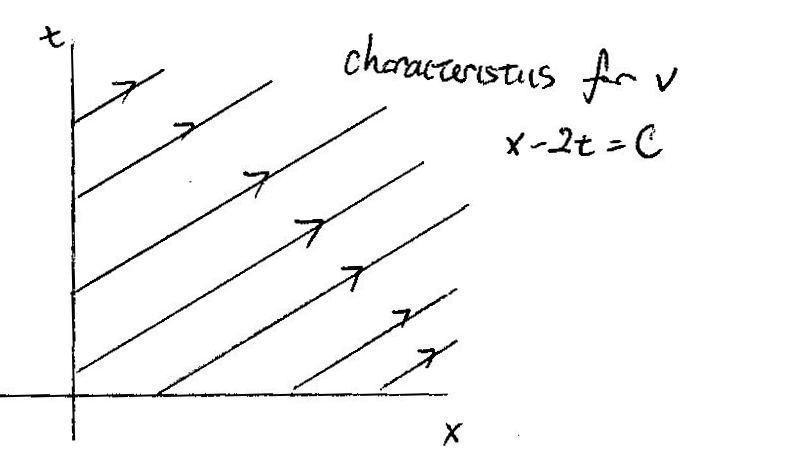
\includegraphics[scale = 0.5]{./_Figures/S098_1.png}
\end{center}
By how $v$ is defined, this corresponds to knowing data about $$u_{t}(x,0) + u_{x}(x, 0)$$ and $$u_{t}(0, t) + u_{x}(0,t).$$
Given $v$, the characteristics for $u_{t} + u_{x} = v$ imply that to solve for $v$, we need to know data about $u(x, 0)$ and $u(0, t)$.
\begin{center}
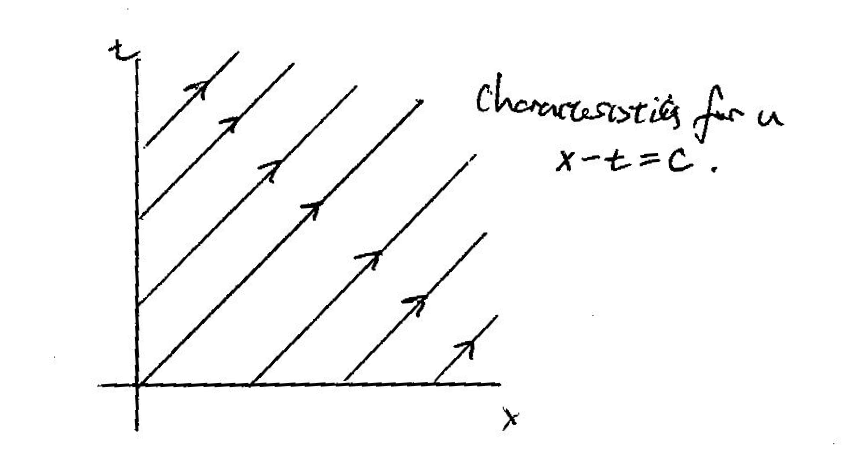
\includegraphics[scale=0.5]{./_Figures/S098_2.png}
\end{center}
Now suppose $u_{tt} + 3u_{xt} + 2u_{xx} = 0$ with
\begin{align*}
u(x,0) &= 0\\
u(0, t) &= 0\\
u_{t}(x, 0) + u_{x}(x, 0) &= 0\\
u_{t}(0, t) + u_{x}(0, t) &= 0.
\end{align*}
Since $v$ is constant on characteristics and $v(x, 0) = v(0, t) = 0$, we have $v = 0$. Since $u(x, 0) = u(0, t) = 0$ and $u$ is constant on characteristics,
$u = 0$. Moreover since the solution is constant on characteristics and we know the values of $u$ when the characteristics hit the $x$ and $t$ axes,
the characteristics uniquely determines the solution and hence $u = 0$ is the unique solution for the boundary value problem.
\hfill\qed

\subsection*{Solution to Spring 2009, \#9}\label{s099}
\subsubsection*{Solution to $(a)$}
Let $E[u] := \frac{1}{2}\int_{D}\abn{\nabla u}^{2}\, dx - \int_{\pr D}(f - \frac{a}{2}u)u\, d\sigma$. Then the minimizer $u$ satisfies
\begin{align*}
0 & = \lim_{\vep \rightarrow 0}\frac{1}{\vep}(E[u + \vep v] - E[u])\\
&= \lim_{\vep \rightarrow 0}\frac{1}{\vep}\bigg(\frac{1}{2}\int_{D}\abn{\nabla u + \vep \nabla v}^{2}\, dx \\
&\hspace{1in}- \int_{\pr D}(f - \frac{a}{2}u - \frac{a}{2}\vep v)(u + \vep v)\, d\sigma - \frac{1}{2}\int_{D}|\nabla u|^{2}\, dx + \int_{\pr D}(f - \frac{a}{2}u)u\, d\sigma\bigg)\\
&= \int_{D}\nabla u \cdot \nabla v\, dx - \int_{\pr D}fv - auv\, d\sigma\\
&= \int_{D}\nabla u \cdot \nabla v\, dx - \int_{\pr D}(f - au)v\, d\sigma\\
&= -\int_{D}\Delta u v\, dx + \int_{\pr D}\bigg(\frac{\pr u}{\pr n} - f + au\bigg)v\, d\sigma
\end{align*}
for all $v$. Then $\Delta u = 0$ in $D$ and $\frac{\pr u}{\pr n} + au = f$ on $\pr D$.
\hfill\qed

\subsubsection*{Solution to $(b)$}
Suppose there were two smooth solutions $u, v$. Let $w:= u - v$. Then
$\Delta w = 0$ in $D$ and $\frac{\pr w}{\pr n} + aw = 0$ on $\pr D$. Thus
\begin{align*}
0 = \int_{D}w\Delta w\, dx = -\int_{D}\abn{\nabla w}^{2}\, dx + \int_{\pr D}\frac{\pr w}{\pr n}w\, d\sigma = \int_{D}\abn{\nabla w}^{2}\, dx - \int_{\pr D}aw^{2}\, d\sigma.
\end{align*}
Since we also are given $a(x) > 0$, we have $\int_{D}\abn{\nabla w}^{2}\, dx \leq 0$. Therefore $w$ is a constant on $D$ and hence $w = 0$. Therefore if a smooth solution exists,
it is unique.
\hfill\qed
